\pdfminorversion=4

\documentclass{beamer}
\usepackage[utf8]{inputenc}
\usepackage[spanish]{babel}
%\usepackage[english]{babel}
\usepackage{graphicx}  % Graphics

\usepackage{beamerthemeULoyola}
\usepackage{graphicx}
\usepackage{booktabs}
\usepackage{blindtext}

%% PRESENTATION CONFIGURATION PARAMETERS %%%%%%%%%%%%%%%%%%%%%%%%%%%%%%%%%%%%%%%
\titlebackgroundfile{images/plantilla_portada}
\framebackgroundfile{images/plantilla_slide}
\definecolor{azulloyola}{HTML}{023E83}
\definecolor{azulloyolaclaro}{HTML}{9497B9}
\definecolor{gris}{HTML}{4C4C4C}
\definecolor{grisclaro}{HTML}{EBEBEB}
\definecolor{examplefrente}{HTML}{218E58}
\definecolor{examplefondo}{HTML}{C2D8CD}
\definecolor{alertfrente}{HTML}{FF0000}
\definecolor{alertfondo}{HTML}{E7BDBD}


\usefonttheme{structurebold}
\setbeamercolor{author in head/foot}{fg=white}
\setbeamercolor{title in head/foot}{fg=white}
\setbeamercolor{section in head/foot}{fg=azulloyola}
\setbeamercolor{normal text}{fg=gris}
\setbeamercolor{frametitle}{fg=azulloyola}
% \setbeamerfont{block title}{size={}}
\setbeamerfont{author}{size=\footnotesize}
\setbeamerfont{date}{size=\footnotesize}
\setbeamertemplate{itemize item}[circle]
\setbeamertemplate{itemize subitem}[triangle]
\setbeamertemplate{itemize subsubitem}[square]
\setbeamertemplate{itemize subsubsubitem}[ball]
\setbeamercolor{itemize item}{fg=azulloyola}
\setbeamercolor{itemize subitem}{fg=azulloyola}
\setbeamercolor{itemize subsubitem}{fg=azulloyola}
\setbeamercolor{itemize subsubsubitem}{fg=azulloyola}
\setbeamercolor{enumerate item}{fg=azulloyola}
\setbeamercolor{enumerate subitem}{fg=azulloyola}
\setbeamercolor{enumerate subsubitem}{fg=azulloyola}
\setbeamercolor{enumerate subsubsubitem}{fg=azulloyola}
% \setbeamercolor{alerted text}{fg=azulloyola}
% \setbeamerfont{alerted text}{series=\bfseries}

\setbeamertemplate{blocks}[shadow=true]
\setbeamercolor*{block title}{bg=azulloyolaclaro,fg=white}
\setbeamercolor*{block body}{bg=grisclaro,fg=gris}

\setbeamercolor*{block title example}{bg=examplefrente,fg=white}
\setbeamercolor*{block body example}{bg=examplefondo,fg=gris}

\setbeamercolor*{block title alerted}{bg=alertfrente,fg=white}
\setbeamercolor*{block body alerted}{bg=alertfondo,fg=gris}

\usecolortheme[named=azulloyola]{structure}


% This command makes that acrobat reader doesn't changes the colors of the slide
% when there are figures with transparencies.
\pdfpageattr {/Group << /S /Transparency /I true /CS /DeviceRGB>>}
%%%%%%%%%%%%%%%%%%%%%%%%%%%%%%%%%%%%%%%%%%%%%%%%%%%%%%%%%%%%%%%%%%%%%%%%%%%%%%%%

%      + Short title.               + Title which appears in the cover.
%      v                            v
\title[Short title]{Diversidad explícita en modelos de Ensembles de Extreme Learning Machine}
%       + Short author names which appear in the slides.
%       v
\author[Author]
{   % Author names which appear in the cover page.
    Carlos Perales-Gonz\'alez\inst{1}
}
%          + Short affiliation which appears in the slides.
%          v
\institute[ULOYOLA]
{   % Affiliation information which appears in the cover page.
    \begin{tabular}{c}
    \inst{1}Universidad Loyola Andaluc\'ia
    \end{tabular}
}
%     + Short acronym of the conference or date of the presentation.
%     v
\date
{   % Conference name which appears in the cover page.
	\today
}

\begin{document}
% Creates the cover page.
\frame{\titlepage}

\begin{frame}{Esquema}
\tableofcontents
\end{frame}


% 45 minutos
\section{Introducción} % 10 minutos

\subsection{Aprendizaje automático (Machine Learning)}
% 1
\frame[allowframebreaks]{\frametitle{Inteligencia artificial. Machine Learning}
	
	\textbf{Ciencia de la Computación}: aquella que estudia el diseño y la construcción de máquinas (computadoras) que resuelven problemas, y cuáles de estos problemas son tratables \cite{mitchell2006discipline}. Dentro de esta Ciencia, un área que acoge cada vez más importante es: el Aprendizaje Automático (\textit{Machine Learning}). \\
	
	\textbf{Aprendizaje Automático (\textit{Machine Learning})}: area de conocimiento que utiliza las Matemáticas para elaborar modelos que estudian qué puede ser predicho a través de los datos, con una serie de hipótesis de modelado, y con qué confiabilidad \cite{mitchell2006discipline}.
	
	\begin{figure}[H]
		\centering
		\label{fig:nested}
		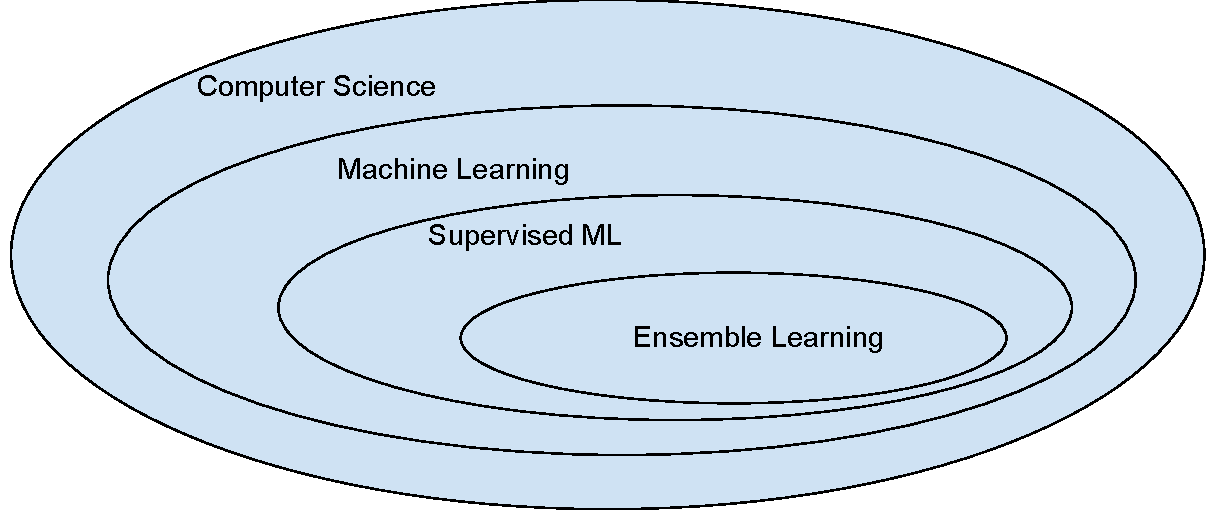
\includegraphics[scale=0.5]{images/nested.pdf}
%		\caption{Explicación del sesgo y la varianza como distancia al centro de una diana}
	\end{figure}

}

\subsection{Categorías del Aprendizaje Automático}

\frame{\frametitle{Machine Learning}

	\begin{itemize}
		\item Supervisado: se infiere una función que relacione variables de entrada (\textit{input variables}) y variables de salida (\textit{targets}), usando datos de situaciones previas donde estos datos pueden ser recogidos \cite{supervised_dict}.
		\begin{itemize}
			\item Regression: target numérico.
			\item Classificación: target categórico.
		\end{itemize}
		\item No supervisado: se infiere la estructura que tiene un conjunto de datos, en ausencia de un target o un feedback \cite{unsupervised_dict}. Los elementos son agrupados siguiendo relaciones entre las variables (\textit{Principal Component Analysis}, \textit{K-means}, $\ldots$).
		\item Por refuerzo:  busca aprender un patrón de comportamiento a través de problemas de toma de decisiones secuenciales con recompensas \cite{reinforcement_dict}.
	\end{itemize}
	
}

\frame[allowframebreaks]{
\frametitle{Supervised Machine Learning}

Conjunto de datos de entrenamiento $\mathcal{D} = \{  (\boldsymbol{x}_1, y_1), \ldots (\boldsymbol{x}_N, y_N) \} = \{ (\boldsymbol{x}_n, y_n) \}_{n=1}^N$. Buscamos un predictor $f : \mathcal{X} \rightarrow \mathcal{Y}$,


	\begin{figure}[H]
	\centering
	\label{fig:f}
	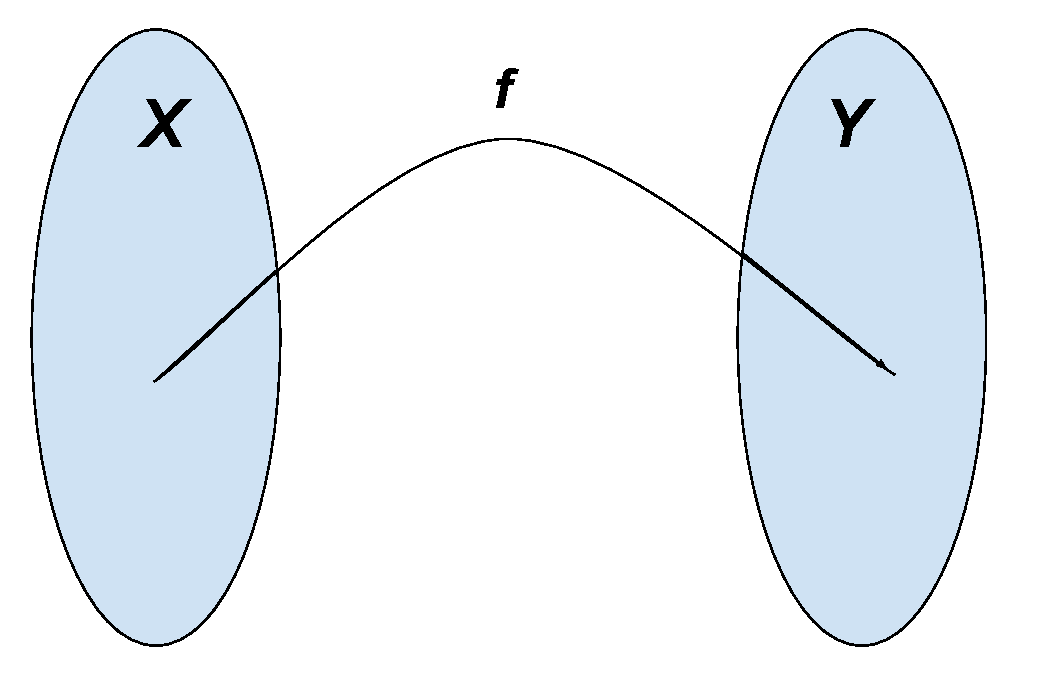
\includegraphics[scale=0.25]{images/f.pdf}
	%		\caption{Explicación del sesgo y la varianza como distancia al centro de una diana}
	\end{figure}

Hay muchos predictores posibles. Además, dependiendo del problema (regresión o clasificación), esa variable $y$ puede ser una variable numérica o categórica. Los problemas de clasificación se pueden convertir en multi-regresión a través del \textit{One-Hot-Encoding} \cite{one_hot_encoding}.


\begin{equation}
\label{eq:onehotencoding}
\boldsymbol{y}_{j, n} =
\begin{cases}
1 & \text{si } j \text{ es la clase a la que pertenece el patrón} n \\
0 & \text{en cualquier otro caso}
\end{cases}
\end{equation}

}
\frame{
En general, no podemos conocer exactamente la relación entre el dominio de las features, $\mathcal{X}$, y el dominio target, $\mathcal{Y}$. Sin embargo, podemos interpolar esos dominios a través de $n=1, \ldots, N$ patrones, con features $\boldsymbol{x}_n \in \mathcal{X}$, y target $\boldsymbol{y}_n \in \mathcal{Y}$.


\begin{equation}
\label{eq:f}
f (\boldsymbol{x}_n; \theta) \approx y_n, \: \forall n .
\end{equation}

Los predictores $f$ dependen de una serie de parámetros $\theta$. Para entrenar un predictor, optimizamos esos parámetros a través de la minimización del error cometido en predecir el set de entrenamiento $\mathcal{D}$.

\begin{equation}
\label{eq:omega_error}
\min_{\theta} \text{ Error} ( \left( f(\boldsymbol{x}_1; \theta ), y_1 \right), \ldots, \left( f(\boldsymbol{x}_N; \theta ), y_N \right) )
\end{equation}
}

\frame{
En problemas de regresión, clásicamente se utiliza el error cuadrático medio, o \textit{Mean Squared Error}, que es equivalente a calcular la norma $L2$ entre el target $y_n, \: n=1, \ldots, N$ y la predicción $f (\boldsymbol{x}_n), \:n=1, \ldots, N$.

\begin{equation}
\label{eq:mse}
\min_{\theta} \frac{1}{N} \sum_{n=1}^{N} { \left( f(\boldsymbol{x}_n; \theta ) - y_1 \right) }^2
\end{equation}


}

\subsection{Dilema sesgo-varianza}

\frame{\frametitle{Definición de sesgo y varianza}

Explicación sesgo

Explicación varianza

}

\frame{\frametitle{Sesgo, varianza y el MSE}
	
	Ecuación matemática con el MSE
	
}

\frame{\frametitle{Ejemplo del sesgo y la varianza}
	
Ejemplo hecho con el Jupyter Notebook
	
}

\section{Ensemble Learning}

\frame{\frametitle{Metodología ensemble}

Motivación a través del sesgo-varianza.

Motivación a través de la diversidad.

}

\frame{\frametitle{Metodología boosting}

Ejemplo de la carrera de caballos (artículo original del Adaboost).

}

\frame{\frametitle{Metodología bagging}
	
Buscar ejemplo
	
}


\frame{\frametitle{Ventajas-desventajas del data sampling}

\textbf{Ventaja:}	
Es fácil de adaptar a cualquier algoritmo. No modifica \textit{la caja negra}, es externo.

\textbf{Desventaja:}
Depende en la heterogeneidad de los datos. Hay que tener muchos datos y que cada subset del conjunto de entrenamiento sea diverso entre sí.

	
}

\frame{\frametitle{Propuestas no data sampling}
	
\begin{itemize}
	\item Diversidad kernel.
	\item Diversidad de parámetros. NCL.
\end{itemize}
	
	
}

\section{Extreme Learning Machine}  % 5 minutos
\frame{\frametitle{Ordinary Least Squares}
}

\frame{\frametitle{Regularized Least Squares}
}

\frame{\frametitle{Extreme Learning Machine}
}




\section{Promoción de la diversidad explícita en ELM}  % 20 minutos
\subsection{RE-ELM}
\subsection{NC-ELM}
\subsection{GNC-ELM}

\section{Conclusiones} % 5 minutos



% END
\section*{END}
\frame{
	\frametitle{END}
\begin{center}
	\huge GRACIAS
\end{center}
}

% BIBLIOGRAPHY
\section*{Bibliography}
\begin{frame}[allowframebreaks]
	\frametitle{References}
    \bibliographystyle{ieeetr}
	\bibliography{references.bib}
\end{frame}


\end{document}
